\setcounter{chapter}{2}

\chapter{函数极限与连续}

极限是微积分理论体系中最基本也最重要的概念之一,后面我们将要讨论的导数(微分)和
积分的概念都是建立在极限概念之上的,更具体地说,导数和定积分都是特定类型的极限。

在上一章学习了数列极限的基础上,本章我们将进一步讨论更具一般性的函数的极限,二者
的定义和性质,从很多方面来看都是相似的,只是由于函数极限的类型更为丰富,相对而言
有关结论也更为多样,有些性质是数列极限所不具备的。

\section{函数极限的概念与性质}

函数极限是我们后续定义导数、积分的概念的基础,因此可以说函数极限的理论也是整个
微积分学的基础。



\section{函数极限的判敛}

\subsection{四则运算}

{\bf 定理3.2.1:}若函数极限存在,则极限运算可以和四则运算交换次序。

{\bf 注:}把握两点
\begin{itemize}
  \setlength{\itemindent}{1cm}
  \item 有限次四则运算
  \item 可以推广到初等函数
\end{itemize}







\subsection{夹逼定理}


\section{无穷大、无穷小和函数的渐近线}

在求解(函数)极限的问题中,分子分母同时趋于零
\ps{所谓不定是相对诸如有界量乘以无穷小(趋于零)、有界量除以无穷大一类容易确定的形式而言的}
(例如:$\limx{0}\df{\cos
x-\cos2x}{x^2}$),或者一个趋于零的函数和一个趋于无穷的函数的乘积(例如:$\limx{+\infty}x^2e^-x$)
的极限通常是较难求解的,这类问题我们称之为“$\df00$”和“$0\cdot\infty$” 型的{\it 不定式(极限)}!


{\bf 思考:}除了“$\df00$”和“$0\cdot\infty$”型的不定式,还可能有其他形式的不定式吗?

{\bf 答:}有,型如:“$\df{\infty}{\infty}$”、“$1^{\infty}$”、“$0^0$”,例如:
$\limx{+\infty}\df{\ln x}{x}$,$\limx{\infty}\left(1+\df1{x}\right)^{\sin
x}$,$\limx{0}x^{2x}$

\subsection{无穷大和无穷小}

{\bf 定义3.3.1:}$f(x)$是$x\to\Delta$时的无穷小$\Leftrightarrow\limx{\Delta}f(x)=0$

{\bf 注:}$\Delta$可任意代表$\infty,\;+\infty,\;-\infty,\;x_0,\;x_0^+,\;x_0^-$之一

{\bf 定理3.3.1-3.3.2}(无穷小的性质)
\begin{enumerate}[(1)]
  \setlength{\itemindent}{1cm}
  \item $\limx{\Delta}f(x)=A\in\mathbb{R}\Leftrightarrow
  f(x)-A$是$x\to\Delta$时的无穷小
  \item $x\to\Delta$时的有界函数与无穷小之积仍为$x\to\Delta$时的无穷小
  \item $x\to\Delta$时的有限个无穷小之和(积)仍为$x\to\Delta$时的无穷小
\end{enumerate}

{\bf 定义3.3.2:}$f(x)$是$x\to\Delta$时的无穷大$\Leftrightarrow\limx{\Delta}\df 1{f(x)}=0$,
可记为:
$$\limx{\Delta}f(x)=\pm\infty$$

{\bf 注:}{\b 无穷大有正负之分!!}

{\bf 【渐近线】}\ps{具体内容请阅读教材自学!}

$x\to x_0$时的无穷大意味着存在{\it 铅直渐近线};$x\to\pm\infty$时的无穷大
{\it 可能}意味着存在{\it 斜渐近线},例如:若$y=f(x)$当$x\to+\infty$时的
存在斜渐近线$y=kx+b$,则
$$k=\limx{+\infty}\df{f(x)}x,\quad b=\limx{+\infty}[f(x)-kx].$$
注意,{\b $x\to\pm\infty$时的斜渐近线可能是不同的!}例如:$y=x\arctan x$趋于
$x\to\pm\infty$时的斜渐近线分别为$y=\pm\df{\pi}2x$.

% {\bf P129-例4:}证明:$x+\sin x$是$x\to\infty$时的无穷大

{\bf 定理3.3.3:}在$x\to\Delta$的同一过程中:
\begin{enumerate}[(1)]
  \setlength{\itemindent}{1cm}
  \item 有界函数与无穷大之和仍为无穷大
  \item 有限个无穷大之乘积仍为无穷大({\it 但可能反号})
\end{enumerate}

{\bf 例:}证明:$f(x)=a_0x^n+a_1x^{n-1}+\ldots+a_n(n\in\mathbb{N})$
是$x\to\infty$时的无穷大,其中:$a_0,a_1,\ldots,a_n\in\mathbb{R},a_0\ne 0$

\begin{shaded}
	{\bf 无穷大之间的比较!}
	
	当$x\to+\infty$时,存在如下的大小关系:设$a>0$,
	$$\ln x<<x^a<<e^x<<\Gamma(x)<<x^x$$
	其中$\Gamma-$函数定义为$\Gamma(x)=\dint_0^{+\infty}t^{x-1}e^{-t}\d t$,
	满足$\Gamma(n)=(n-1)!,\;(n\in\mathbb{Z}_+)$
\end{shaded}

\subsection{无穷小的比较}



\subsection{斜渐近线}

若$y=f(x)$当$x\to+\infty$时以$y=kx+b$为斜渐进线,则有
$$k=\limx{+\infty}\df{f(x)}{x}=k,\quad b=\limx{+\infty}[f(x)-kx]$$

{\bf 例:}求曲线$y^2-x^2=2x$的渐近线。

{\bf 教材3.3.4节-例10:}求函数$f(x)=\df{2x^2-3}{x+1}$的渐近线。

\begin{center}
	\resizebox{!}{5cm}{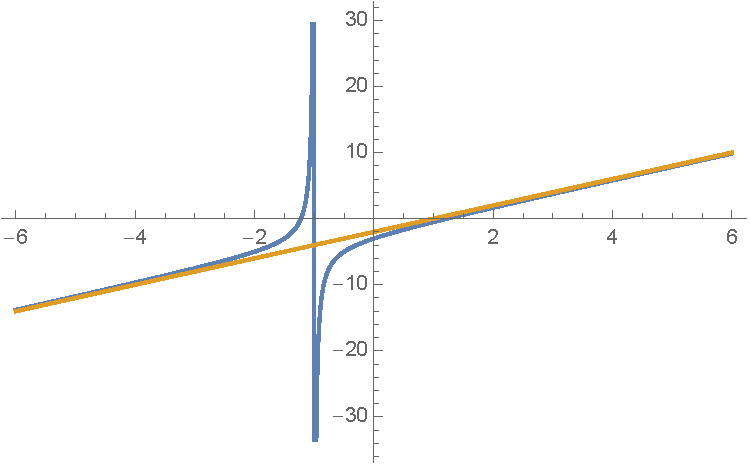
\includegraphics{./images/ch3/asyx.pdf}}
\end{center}

\section{函数的连续性}



\subsection{基本性质}

{\bf 定理3.4.1-3.4.4:}


\subsection{连续函数在有界闭区间上的性质}

\subsubsection{【最值定理】}


\subsubsection{【介值定理】}



% \section*{补充例题}
% \addcontentsline{toc}{section}{补充例题}
% 
% {\bf 例}:证明函数$f(x)=\left\{\begin{array}{ll}
% x,\;&x\in\mathbb{Q}\\ 0,\;&\mathrm{else}
% \end{array}\right.$
% 仅在$x=0$连续
% 
% {\bf 证:}显然$f(0)=0$。注意到
% $$0<|f(x)|\leq |x|,$$
% 而$\lim\limits_{x\to 0}|x|=0$,故由夹逼定理
% $$\lim\limits_{x\to 0}f(x)=0=f(0),$$
% 也即$f(x)$在$x=0$连续。
% 
% \bigskip
% 
% 设$x_0\ne 0$,下证$\lim\limits_{x\to x_0}f(x)$不存在,进而可知
% $f(x)$在$x_0$处不连续。事实上,若设$\lim\limits_{x\to x_0}f(x)$存在,
% 则
% $$\lim\limits_{x\to x_0}D(x)=\frac{\lim\limits_{x\to x_0}f(x)}
% {\lim\limits_{x\to x_0}x}$$
% 也存在,从而与$D(x)$在任意点处极限不存在矛盾。
% 
% 综上,$f(x)$仅在$x=0$连续。
% 
% \newpage
% 
% \newpage



\newpage

\section*{课后作业}
\addcontentsline{toc}{section}{课后作业}

{\bf 【必作题】}

\begin{itemize}
  \item 习题3.1:4(1,3),7,15
  \item 习题3.2:2,3,4,5
  \item 习题3.3:2,4,5,7(2,6),8,9,10(3,4)
  \item 习题3.4:5(1-3),9,15,17
\end{itemize}

\bigskip

\hrule

\bigskip
\bigskip

{\bf 【思考题】}
\begin{itemize}
  \item 习题3.1:10,11,12
  \item 习题3.2:6,7
  \item 证明:$$\limn\left\{\lim\limits_{m\to\infty}\left[\cos^{2m}(n!\pi
	x)\right]\right\}=D(x)$$
	其中$D(x)$为Dirichlet函数
%   \item 自学3.3.3节:渐近线 
  \item 习题3.3:1,6,12,13
  \item  计算极限
  \item 习题3.4:1,3,13,14,16,19
  \item 设$a_1<a_2<\ldots<a_n$,证明以下方程有$n-1$个实根
	$$\df 1{x-a_1}+\df 1{x-a_2}+\ldots+\df 1{x-a_n}=0.$$
\end{itemize}

\newpage

\section*{补充例题}
\addcontentsline{toc}{section}{补充例题}



{\bf 例:}设$f(x)$在$x_0$的某邻域内有定义,且$x_0$为其间断点,则下列函数
必以$x_0$为间断点的是(B)

\quad
(A)\;$f(x)\sin x$\hspace{2cm}
(B)\;$f(x)+\sin x$\hspace{2cm}
(C)\;$f^2(x)$\hspace{2cm}
(D)\;$|f(x)|$ 

{\bf 例:}设$x\to 0$时,$e^{\tan x}-e^x$与$x^n$为同阶无穷小,则$n$=(C)
\ps{Taylor展开}

\quad
(A)\;$1$\hspace{2cm}
(B)\;$2$\hspace{2cm}
(C)\;$3$\hspace{2cm}
(D)\;$4$ 

{\bf 例:}设$x\to 0$时,$x-\sin ax$与$x^2\ln(1-bx)$为同阶无穷小,则(A)
\ps{Taylor展开}

\quad
(A)\;$a=1,b=-\df16$\hspace{1em}
(B)\;$a=1,b=\df16$\hspace{1em}
(C)\;$a=-1,b=-\df16$\hspace{1em}
(D)\;$a=-1,b=\df16$

{\bf 例:}若$f(x)=\df{\sqrt[3]{x}}{\lambda-e^{-kx}}$在$(-\infty,+\infty)$
上连续,且$\limx{+\infty}f(x)=0$,则(D)

\quad
(A)\;$\lambda<0,k<0$\hspace{1cm}
(B)\;$\lambda<0,k>0$\hspace{1cm}
(C)\;$\lambda\geq0,k<0$\hspace{1cm}
(D)\;$\lambda\leq0,k>0$

% \begin{tabbing}
% 	\hspace{3cm}\=\hspace{3cm}\=\hspace{3cm}\=\kill
% 	\quad\quad\quad
% 	(A)\;$\lambda<0,k<0$\>  
% 	\quad\quad\quad
% 	(B)\;$\lambda<0,k>0$\>
% 	\quad\quad\quad  
% 	(C)\;$\lambda\geq0,k<0$\>
% 	\quad\quad\quad 
% 	(D)\;$\lambda\leq0,k>0$
% \end{tabbing} 

{\bf 例:}设$f(x)$在$(a,b)$内均有定义且单调有界,则$f(x)$在$(a,b)$内的间断点类型只能是(C)
\begin{tabbing}
	\hspace{8cm}\=\kill
	\quad\quad\quad
	(A)\;可去间断点 \> 
	(B)\;第二类间断点 \\ 
	\quad\quad\quad
	(C)\;跳跃间断点\>
	(D)\;不能确定
\end{tabbing}



{\bf 例:}



{\bf 例:}设$x\in(0,1]$时,$f(x)=x^{\sin x}$,且对任意$x$
$$f(x)+k=2f(x+1),$$
求常数$k$的值,使得极限$\limx0f(x)$存在。

[提示]:易知$\limx{0^+}f(x)=1$,有$x\in(-1,0]$时,
$$f(x)=2(x+1)^{\sin(x+1)}-k,$$
故$\limx{0^-}f(x)=2-k$,从而可得$k=1$.

{\bf 例:}设$f(x)$在$[a,b]$上连续,$\{x_n\}$为$[a,b]$上任一数列,求
$\limn\sqrt[n]{\df1n\sum\limits_{k=1}^ne^{f(x_k)}}$

[提示]:$e^{f(x)}$在$[a,b]$上连续且非负,故可设$m,M$分别为其在$[a,b]$上的最大和最小值,
从而由夹逼定理
$$\sqrt[n]m\leq\sqrt[n]{\df1n\sum\limits_{k=1}^ne^{f(x_k)}}\leq\sqrt[n]M,$$
由此易知原式$=1$。
